\documentclass{beamer}
\usetheme{Boadilla}

\makeatother
\setbeamertemplate{footline}
{
    \leavevmode%
    \hbox{%
    \begin{beamercolorbox}[wd=.4\paperwidth,ht=2.25ex,dp=1ex,center]{author in head/foot}%
        \usebeamerfont{author in head/foot}\insertshortauthor
    \end{beamercolorbox}%
    \begin{beamercolorbox}[wd=.55\paperwidth,ht=2.25ex,dp=1ex,center]{title in head/foot}%
        \usebeamerfont{title in head/foot}\insertshorttitle
    \end{beamercolorbox}%
    \begin{beamercolorbox}[wd=.05\paperwidth,ht=2.25ex,dp=1ex,center]{date in head/foot}%
        \insertframenumber{}
    \end{beamercolorbox}}%
    \vskip0pt%
}
\makeatletter
\setbeamertemplate{navigation symbols}{}

\usepackage[T1]{fontenc}
\usepackage{lmodern}
\usepackage{amssymb,amsmath,bm}
\renewcommand{\familydefault}{\sfdefault}

\DeclareMathOperator*{\Cov}{Cov}

\usepackage{mathtools}
\usepackage{graphicx}
\usepackage{threeparttable}
\usepackage{booktabs}
\usepackage{siunitx}
\sisetup{parse-numbers=false}

% \setlength{\OuterFrameSep}{-2pt}
% \makeatletter
% \preto{\@verbatim}{\topsep=-10pt \partopsep=-10pt }
% \makeatother

\title[Week 2:\ R Tutorial]{Week 2:\ R Tutorial}
\author[ResEcon 703:\ Advanced Econometrics]{ResEcon 703:\ Topics in Advanced Econometrics}
\date{Matt Woerman\\University of Massachusetts Amherst}

\begin{document}

{\setbeamertemplate{footline}{} 
\begin{frame}[noframenumbering]
    \titlepage
\end{frame}
}

\begin{frame}\frametitle{Agenda}
    Last week
    \begin{itemize}
        \item Structural estimation
    \end{itemize}
    \vspace{2ex}
    This week's topics
    \begin{itemize}
    	\item \hyperlink{page.\getpagerefnumber{resources}}{R resources}
        \item \hyperlink{page.\getpagerefnumber{objects}}{Objects in R}
        \item \hyperlink{page.\getpagerefnumber{functions}}{Functions and packages in R}
        \item \hyperlink{page.\getpagerefnumber{math}}{Math and statistics in R}
        \item \hyperlink{page.\getpagerefnumber{data}}{Data in R}
        \item \hyperlink{page.\getpagerefnumber{examples}}{R Examples}
    \end{itemize}
    \vspace{2ex}
    This week's ``reading''
    \begin{itemize}
        \item R \texttt{swirl} interactive tutorials
    \end{itemize}
\end{frame}

\section{R Resources}
\label{resources}
\begin{frame}\frametitle{}
    \vfill
    \centering
    \begin{beamercolorbox}[center]{title}
        \Large R Resources
    \end{beamercolorbox}
    \vfill
\end{frame}

\begin{frame}\frametitle{Hat Tips}
    This lecture is inspired heavily by notes and slides created by
    \begin{itemize}
        \item \href{https://www.fionaburlig.com/}{Fiona Burlig, University of Chicago}
        \item \href{https://grantmcdermott.com/}{Grant McDermott, University of Oregon}
        \item \href{http://edrub.in/}{Ed Rubin, University of Oregon}
    \end{itemize}
    \vspace{3ex}
    Many thanks to them for generously making their course materials available online for all!
\end{frame}

\begin{frame}\frametitle{Installing R}
    Installing R is \emph{usually} straightforward \\
    \vspace{1ex}
    \begin{tabular}{@{\extracolsep{-2ex}} c l}
        \begin{tabular}{c}
            
\includegraphics[width=0.05\linewidth]{r}
        \end{tabular} & 
        \begin{tabular}{l}
            \parbox{0.9\linewidth}{
            \href{https://cran.r-project.org/}{Download (\texttt{cran.r-project.org})} and install R
            }
        \end{tabular}
    \end{tabular} \\
    \vspace{1ex}
    \begin{tabular}{@{\extracolsep{-2ex}} c l}
        \begin{tabular}{c}
            
\includegraphics[width=0.05\linewidth]{rstudio}
        \end{tabular} & 
        \begin{tabular}{l}
            \parbox{0.9\linewidth}{
            \href{https://www.rstudio.com/products/rstudio/download/}{Download (\texttt{www.rstudio.com/products/rstudio/download})}\\ and install RStudio Desktop (Open Source License)
            }
        \end{tabular}
    \end{tabular} \\
    \vspace{3ex}
    What is the difference between R and RStudio? \\
    \vspace{1ex}
    \begin{tabular}{@{\extracolsep{-2ex}} c l}
        \begin{tabular}{c}
            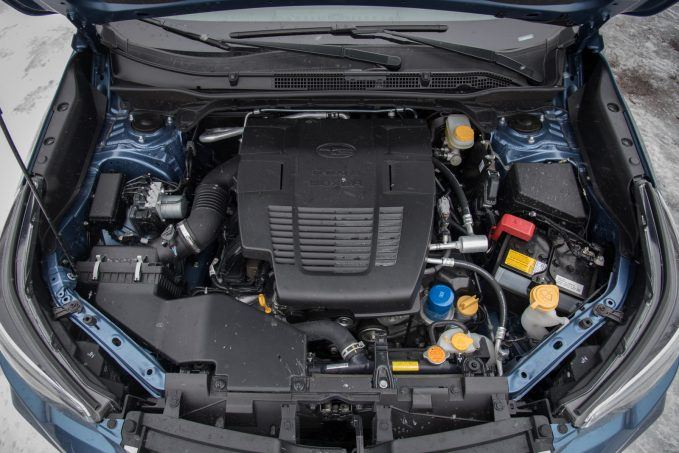
\includegraphics[width=0.25\linewidth]{engine}
        \end{tabular} & 
        \begin{tabular}{l}
            \parbox{0.65\linewidth}{
            R is like a car's engine. It is the program that powers your data analysis.
            }
        \end{tabular}
    \end{tabular} \\
    \vspace{1ex}
    \begin{tabular}{@{\extracolsep{-2ex}} c l}
        \begin{tabular}{c}
            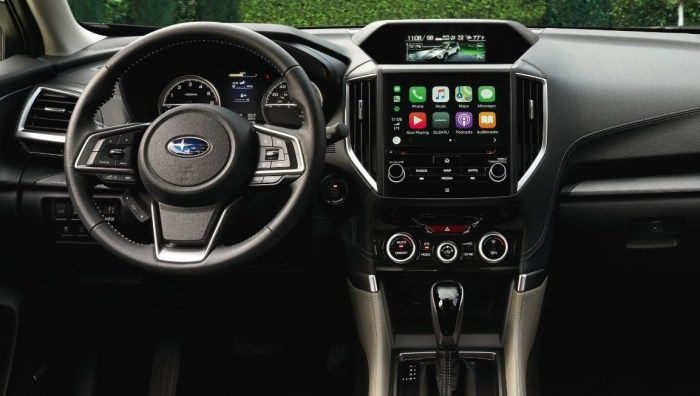
\includegraphics[width=0.25\linewidth]{dashboard}
        \end{tabular} & 
        \begin{tabular}{l}
            \parbox{0.65\linewidth}{
            RStudio is like a car's dashboard. It is the program you interact with to harness the power of your ``engine.''
            }
        \end{tabular}
    \end{tabular}
\end{frame}

\begin{frame}[fragile]\frametitle{R \texttt{swirl} Interactive Tutorials}
    \texttt{swirl} is an R package that interactively teaches you how to use R
    \begin{itemize}
    	\item Information available here: \href{https://swirlstats.com/}{\texttt{swirlstats.com}}
    \end{itemize}
    \vspace{2ex}
    <<R CODE HERE>>
    \vspace{2ex}
    These three \texttt{swirl} tutorials (R Programming, Getting and Cleaning Data, and Advanced R Programming) introduce the main R concepts we will use in this course
\end{frame}

\begin{frame}\frametitle{More R Resources}
    These links provide a variety of perspectives and topics related to using R for statistical analysis, all of which may be useful as you learn to use R for structural estimation in this course
    \begin{itemize}
        \item \href{https://www.datacamp.com/courses/free-introduction-to-r}{DataCamp's Introduction to R}
        \item \href{https://r4ds.had.co.nz/}{R for Data Science book}
        \item \href{https://adv-r.hadley.nz/}{Advanced R book}
        \item \href{https://github.com/edrubin/EC525S19}{Ed Rubin's Econometrics lab slides}
        \item \href{http://edrub.in/ARE212/notes.html}{Ed Rubin's Econometrics section notes}
        \item \href{https://www.fionaburlig.com/teaching/are212}{Fiona Burlig's Econometrics section notes} (warning: puns ahead)
        \item \href{https://github.com/uo-ec607/lectures}{Grant McDermott's Data Science for Economists lecture slides}
    \end{itemize}
\end{frame}

\begin{frame}\frametitle{Some Complements to R}
    \LaTeX\ and \texttt{knitr}
    \begin{itemize}
        \item \href{https://www.latex-project.org/}{\LaTeX\ (\texttt{www.latex-project.org})}: Typesetting system with great functionality for technical and scientific documents
        \item \href{https://yihui.name/knitr/}{\texttt{knitr} (\texttt{yihui.name/knitr})}: R package that integrates R code and output into \LaTeX\ documents (or HTML, Markdown, etc.)
    \end{itemize}
    \vspace{3ex}
    Git, GitHub, and SmartGit
    \begin{itemize}
        \item \href{https://git-scm.com/}{Git (\texttt{git-scm.com})}: Version control system
        \item \href{https://github.com/}{GitHub (\texttt{github.com})}: Hosting platform for Git
        \begin{itemize}
            \item Some alternatives exist: BitBucket, SourceForge, GitLab
        \end{itemize}
        \item \href{https://www.syntevo.com/smartgit/}{SmartGit (\texttt{www.syntevo.com/smartgit})}: GUI client for Git
        \begin{itemize}
            \item Many alternatives exist: GitHub Desktop, GitKraken, SourceTree
        \end{itemize}
    \end{itemize}
\end{frame}

\section{Objects in R}
\label{objects}
\begin{frame}\frametitle{}
    \vfill
    \centering
    \begin{beamercolorbox}[center]{title}
        \Large Objects in R
    \end{beamercolorbox}
    \vfill
\end{frame}

\begin{frame}[fragile]\frametitle{Object Basics}
    Everything is an object, and every object has a name and value
    <<R CODE HERE>>
\end{frame}

\begin{frame}\frametitle{Classes, Types, and Structures}
    Every object has a type
    \begin{itemize}
        \item Numeric: \texttt{1}, \texttt{0.5}, \texttt{2/3}, \texttt{pi}
        \item Character: \texttt{"Hello"}, \texttt{"cruel world"}, \texttt{"Metrics is fun!"}
        \item Logical: \texttt{TRUE}, \texttt{FALSE}, \texttt{T}, \texttt{F}
    \end{itemize}
    \vspace{2ex}
    Every object has a structure
    \begin{itemize}
        \item Vector
        \item Matrix
        \item List
        \item Data frame
    \end{itemize}
    \vspace{2ex}
    \texttt{class()}, \texttt{typeof()}, \texttt{str()} give information about an object
\end{frame}

\begin{frame}[fragile]\frametitle{Vectors}
    A vector is a collection of elements of the same type
    \begin{itemize}
        \item \texttt{c()} combines elements into a vector
        \item \texttt{seq()} and \texttt{:} create sequential vectors of numeric elements
    \end{itemize}
    <<R CODE HERE>>
    \vspace{2ex} 
    If you combine elements of different types, R will convert some
    <<R CODE HERE>>
\end{frame}

\begin{frame}[fragile]\frametitle{Matrices}
    A matrix is a collection of elements of the same type arranged in two dimensions \\
    \vspace{3ex}
    \texttt{matrix()} arranges a vector of data into a matrix
    \begin{itemize}
        \item \texttt{data}: Vector of data to create matrix
        \item \texttt{nrow} or \texttt{ncol}: Number of rows or columns in the matrix
        \item \texttt{byrow}: Logical indicating how to arrange data
    \end{itemize}
    <<R CODE HERE>>
\end{frame}

\begin{frame}[fragile]\frametitle{Lists}
    A list is a collection of elements that can have different types and different structures \\
    \vspace{3ex}
    \texttt{list()} combines elements into a list
    <<R CODE HERE>>
\end{frame}

\begin{frame}[fragile]\frametitle{Data Frames}
    A data frame is a structured table of data arranged in two dimensions
    \begin{itemize}
        \item Each column is a ``variable'' and each row is an ``observation''
        \item Technically, a data frame is a list of named vectors of the same length
        \begin{itemize}
            \item Each vector is a ``variable''
            \item The length of each vector equals the number of ``observations''
        \end{itemize}
    \end{itemize}
    \vspace{3ex}
    \texttt{data.frame()} combines vectors into a data frame
    <<R CODE HERE>>
\end{frame}

\section{Functions and Packages in R}
\label{functions}
\begin{frame}\frametitle{}
    \vfill
    \centering
    \begin{beamercolorbox}[center]{title}
        \Large Functions and Packages in R
    \end{beamercolorbox}
    \vfill
\end{frame}

\begin{frame}\frametitle{Functions}
    A function in R
    \begin{enumerate}
        \item Takes some inputs
        \item Performs some internal tasks
        \item Returns some output
    \end{enumerate}
    \vspace{2ex}
    We have already seen some examples of functions
    \begin{itemize}
        \item \texttt{matrix()}
        \begin{enumerate}
            \item Takes a vector of data, information about the size of the matrix, and information about the arrangement of the matrix
            \item Arranges the data in the way specified by the other inputs
            \item Returns a matrix object
        \end{enumerate}
    \end{itemize}
    \vspace{2ex}
    Use \texttt{?} (e.g., \texttt{?matrix}) to get the help file for a function
\end{frame}

\begin{frame}[fragile]\frametitle{Function Inputs}
    Many functions have default inputs so you do not have to specify all the arguments
    \begin{itemize}
        \item These defaults are shown when you look at the function help file
    \end{itemize}
    \vspace{2ex}
    Use \texttt{?matrix} to see the set of default inputs for the \texttt{matrix()} function
    <<R CODE HERE>>
    \vspace{2ex}
    So the default inputs would create a 1 $\times$ 1 matrix of \texttt{NA}
    <<R CODE HERE>>
    \vspace{2ex}
    Inputs can also be highly flexible
    \begin{itemize}
        \item \texttt{c()} allows for any number of arguments (as long as you have the memory to create a vector of the specified length)
    \end{itemize}
\end{frame}

\begin{frame}\frametitle{User-Defined Functions}
    R makes it easy to define your own functions \\
    \vspace{2ex}
    Why create your own functions?
    \begin{itemize}
        \item You are performing the same task more than once
        \item You want to make it easier to parallelize your code
        \item You want to make your code more readable
    \end{itemize}
    \vspace{2ex}
    How to create your own functions using \texttt{function()\char '173 \char '175}
    \begin{enumerate}
        \item Specify the inputs in the \texttt{()}
        \item Write the code for the function tasks in the \texttt{\char '173 \char '175}
        \item Specify the output using \texttt{return()} in the \texttt{\char '173 \char '175}
    \end{enumerate}
\end{frame}

\begin{frame}[fragile]\frametitle{Function Example}
    Make a function that calculates the mean sum of squares of three numbers \\
    <<R CODE HERE>>
    \vspace{1ex}
    Try it out
    <<R CODE HERE>>
    \vspace{1ex}
    What if we want a default argument?
    <<R CODE HERE>>
    \vspace{1ex}
    What if we want a flexible number of inputs?
    \begin{itemize}
        \item That is a little more complicated and context-specific\ldots
    \end{itemize}
\end{frame}

\begin{frame}\frametitle{Packages}
    A package is a bundle of code, documentation, and data that has been created and distributed by another R user
    \begin{itemize}
        \item More than 16,000 packages are available on CRAN, the official repository of R packages 
    \end{itemize}
    \vspace{2ex}
    What is so great about packages?
    \begin{itemize}
        \item Packages greatly increase the functionality available to you through ``canned'' routines
        \item Packages are open source
        \begin{itemize}
            \item A package can be created by anyone, even you!
            \item You can see the source code in any package
        \end{itemize}
        \item Some packages have vignettes that provide detailed examples for using the package's functionality
    \end{itemize}
    \vspace{2ex}
    Any problems to be aware of?
    \begin{itemize}
        \item A package can be created by anyone, so \emph{caveat utilitor} (user beware)
    \end{itemize}
\end{frame}

\begin{frame}[fragile]\frametitle{Using Packages}
    First download a package from CRAN using \texttt{install.packages()}
    <<R CODE HERE>>
    \vspace{3ex}
    Then load the package into your R session using \texttt{library()}
    <<R CODE HERE>>
    \vspace{3ex}
    Update packages occasionally using \texttt{update.packages()}
\end{frame}

\begin{frame}\frametitle{Recommended Packages}
    Packages we will use in this course
    \begin{itemize}
        \item \texttt{tidyverse}
        \begin{itemize}
            \item Collection of packages that improve data analysis and visualization
        \end{itemize}
        \item \texttt{mlogit}
        \begin{itemize}
            \item Estimating multinomial logit models
        \end{itemize}
        \item \texttt{gmm}
        \begin{itemize}
            \item Generalized method of moments estimation
        \end{itemize}
    \end{itemize}
    \vspace{0.5ex}
    Other good packages
    \begin{itemize}
        \item \texttt{glue}
        \begin{itemize}
            \item Character functions
        \end{itemize}
        \item \texttt{lubridate}
        \begin{itemize}
            \item Date and time functions
        \end{itemize}
        \item \texttt{lfe}
        \begin{itemize}
            \item Fixed effects models
        \end{itemize}
        \item \texttt{furrr}
        \begin{itemize}
            \item Parallelization
        \end{itemize}
    \end{itemize}
\end{frame}

\section{Math and Statistics in R}
\label{math}
\begin{frame}\frametitle{}
    \vfill
    \centering
    \begin{beamercolorbox}[center]{title}
        \Large Math and Statistics in R
    \end{beamercolorbox}
    \vfill
\end{frame}

\begin{frame}[fragile]\frametitle{Math Operations}
    <<R CODE HERE>>
\end{frame}

\begin{frame}[fragile]\frametitle{Math Functions}
    <<R CODE HERE>>
\end{frame}

\begin{frame}[fragile]\frametitle{Statistics Functions}
    <<R CODE HERE>>
\end{frame}

\begin{frame}[fragile]\frametitle{Sampling Functions}
    <<R CODE HERE>>
\end{frame}

\begin{frame}[fragile]\frametitle{Vectorization}
    Many operations and functions are applied to each element of a vector
    <<R CODE HERE>>
\end{frame}

\begin{frame}[fragile]\frametitle{Vector Math}
    You can also operate on vectors elementwise
    <<R CODE HERE>>
    \vspace{3ex}
    But weird things can happen if the vectors are different lengths
    <<R CODE HERE>>
\end{frame}

\begin{frame}[fragile]\frametitle{Indexing Vectors}
    Access elements within a vector using \texttt{[]}
    <<R CODE HERE>>
\end{frame}

\begin{frame}[fragile]\frametitle{Matrices as Vectors}
    Matrices (usually) work like vectors
    <<R CODE HERE>>
\end{frame}

\begin{frame}[fragile]\frametitle{Matrix Addition}
    Matrix addition and subtraction is performed elementwise
    <<R CODE HERE>>
\end{frame}

\begin{frame}[fragile]\frametitle{Matrix Multiplication}
    Using \texttt{*} to multiply matrices performs elementwise multiplication
    <<R CODE HERE>>
    \vspace{3ex}
    You must use \texttt{\%*\%} to get the matrix product
    <<R CODE HERE>>
\end{frame}

\begin{frame}[fragile]\frametitle{Matrix Functions}
    R has many other functions for use with matrices
    <<R CODE HERE>>
\end{frame}

\begin{frame}[fragile]\frametitle{Indexing Matrices}
    Access elements within a matrix using \texttt{[]}
    <<R CODE HERE>>
\end{frame}

\section{Data in R}
\label{data}
\begin{frame}\frametitle{}
    \vfill
    \centering
    \begin{beamercolorbox}[center]{title}
        \Large Data in R
    \end{beamercolorbox}
    \vfill
\end{frame}

\begin{frame}[fragile]\frametitle{Example Data Frame}
    You will mostly interact with datasets in the form of data frames
    \begin{itemize}
        \item R includes several example data frames
    \end{itemize}
    <<R CODE HERE>>
\end{frame}

\begin{frame}[fragile]\frametitle{Indexing Data Frames}
    Access elements within a data frame using \texttt{[]}
    <<R CODE HERE>>
    \vspace{2ex}
    Access a variable of a data frame using \texttt{\$}
    <<R CODE HERE>>
\end{frame}

\begin{frame}[fragile]\frametitle{Adding New Variables}
    You may want to add new variables to a data frame
    <<R CODE HERE>>
    But that can get a little clunky. Is there a better way?
\end{frame}

\begin{frame}\frametitle{\texttt{dplyr}}
    \texttt{dplyr} is a package that greatly improves data manipulation in R
    \begin{itemize}
        \item Part of the \texttt{tidyverse} so it is already installed and loaded from earlier code
    \end{itemize}
    \vspace{3ex}
    \texttt{dplyr} is a ``grammar of data manipulation''
    \begin{itemize}
        \item Data compose the subjects of your analysis
        \item \texttt{dplyr} provides the the verbs
        \begin{itemize}
            \item \texttt{mutate()}: Adds new variables
            \item \texttt{select()}: Picks variables
            \item \texttt{filter()}: Picks observations
            \item \texttt{arrange()}: Changes the order of observations
            \item \texttt{summarize()} or \texttt{summarise()}: Summarizes multiple observations
        \end{itemize}
    \end{itemize}
\end{frame}

\begin{frame}[fragile]\frametitle{Adding New Variables with \texttt{dplyr}}
    \texttt{mutate(.data, \ldots)}
    \begin{itemize}
        \item \texttt{.data}: Existing data frame
        \item \texttt{\ldots}: Names and values of new variables
    \end{itemize}
    <<R CODE HERE>>
\end{frame}

\begin{frame}\frametitle{Tibbles}
    \texttt{tidyverse} also introduces a new kind of data frame, the tibble
    \begin{itemize}
        \item Actually, \texttt{tibble} is the name of the package that has the code to create and manipulate objects of class \texttt{tbl\_df}
        \item But it is easier to say ``tibble,'' so that is what users call both the package and the object
        \item I will probably use ``tibble'' and  ``data frame'' interchangeably to mean ``tibble''
    \end{itemize}
    \vspace{2ex}
    Why are tibbles better than data frames?
    \begin{itemize}
        \item Data frames sometimes exhibit weird behaviors related to naming variables or trying to convert variable types
        \item Tibbles are smarter about how much data they show you when you call them
        \begin{itemize}
            \item You do not have to use \texttt{head()} to supress output
        \end{itemize}
    \end{itemize}
\end{frame}

\begin{frame}[fragile]\frametitle{Example Tibble}
    \texttt{dplyr} comes with several examples tibbles
    <<R CODE HERE>>
    \vspace{1ex}
    Let's play around with the \texttt{dplyr} verbs on this tibble
\end{frame}

\begin{frame}[fragile]\frametitle{\texttt{select()} Example}
    <<R CODE HERE>>
\end{frame}

\begin{frame}[fragile]\frametitle{\texttt{filter()} Example}
    <<R CODE HERE>>
\end{frame}

\begin{frame}[fragile]\frametitle{\texttt{arrange()} Example}
    <<R CODE HERE>>
\end{frame}

\begin{frame}[fragile]\frametitle{Multiple \texttt{dplyr} Functions}
    Nest functions inside one another to perform multiple functions
    <<R CODE HERE>>
    \vspace{1ex}
    But either option can get very difficult to read and understand
\end{frame}

\begin{frame}[fragile]\frametitle{Pipes}
    Pipes make a sequence of functions or operations much more readable
    \begin{itemize}
        \item Put each new step on its own line rather than all together
        \item Start with the first step rather than working inside-out
    \end{itemize}
    \vspace{2ex}
    \texttt{x \%>\% f(y)} is the same as \texttt{f(x, y)}
    <<R CODE HERE>>
\end{frame}

\begin{frame}[fragile]\frametitle{Multiple \texttt{dplyr} Functions Using Pipes}
    Let's do the same sequence of three functions but using pipes
    <<R CODE HERE>>
\end{frame}

\begin{frame}[fragile]\frametitle{\texttt{summarize()} Example}
    \texttt{summarize()} applies a function to a group of observations
    \begin{itemize}
        \item \texttt{group\_by()} specifies the grouping to use
    \end{itemize}
    <<R CODE HERE>>
\end{frame}

\begin{frame}[fragile]\frametitle{\texttt{NA} and Other Special Values}
    R has several special values to indicate non-standard objects or elements
    \begin{itemize}
        \item \texttt{NA}: Missing value
        \item \texttt{NaN}: Not a number
        \item \texttt{NULL}: ``Undefined''
        \item \texttt{Inf} and \texttt{-Inf}: $\infty$ and $-\infty$
    \end{itemize}
\end{frame}

\begin{frame}[fragile]\frametitle{Skipping \texttt{NA}s}
    The argument \texttt{na.rm = TRUE} skips missing values
    <<R CODE HERE>>
\end{frame}

\section{R Examples}
\label{examples}
\begin{frame}\frametitle{}
    \vfill
    \centering
    \begin{beamercolorbox}[center]{title}
        \Large R Examples
    \end{beamercolorbox}
    \vfill
\end{frame}

\begin{frame}\frametitle{OLS Regression in R}
    Using the \texttt{mtcars} dataset, regress \texttt{mpg} on \texttt{hp}
    $$\texttt{mpg}_i = \beta_0 + \beta_1 \texttt{hp}_i + \varepsilon_i$$ \\
    \vspace{2ex}
    Perform this simple linear OLS regression three ways:
    \begin{enumerate}
        \item ``Canned'' \texttt{lm()} function
        \item ``Hand-coded'' OLS estimators
        \item User-defined OLS function 
    \end{enumerate}
    \vspace{2ex}
    Report parameter estimates, standard errors, t stats, and p values \\
    \vspace{2ex}
    But before running a regression...
\end{frame}

\begin{frame}[fragile]\frametitle{Look at the \texttt{mtcars} Dataset}
    You should always double-check the structure of your dataset
    <<R CODE HERE>>
\end{frame}

\begin{frame}[fragile]\frametitle{Summarize the \texttt{mtcars} Dataset}
    It can be helpful to generate basic summary statistics for your dataset to get a sense for the scale and variation of each variable
    <<R CODE HERE>>
\end{frame}

\begin{frame}[fragile]\frametitle{Plot the \texttt{mtcars} Dataset}
    Plotting the data can give an idea of what to expect from your regression
    <<R CODE HERE>>
\end{frame}

\begin{frame}[fragile]\frametitle{Regression Using \texttt{lm()} Function}
    The \texttt{lm()} function fits a linear model to a dataset
    \begin{itemize}
        \item To see how to use the \texttt{lm()} function, type \texttt{?lm}
    \end{itemize}
    <<R CODE HERE>>
    \vspace{2ex}
    The \texttt{lm()} function requires a \texttt{formula} object
    \begin{itemize}
        \item \texttt{y} {\raise.17ex\hbox{$\scriptstyle\mathtt{\sim}$}} $\mathtt{x1 + x2 + x3}$ regresses variable \texttt{y} on variables \texttt{x1}, \texttt{x2}, and \texttt{x3}
    \end{itemize}
\end{frame}

\begin{frame}[fragile]\frametitle{Regression Using \texttt{lm()} Function}
	\vspace{-3ex}
    $$\texttt{mpg}_i = \beta_0 + \beta_1 \texttt{hp}_i + \varepsilon_i$$
    \vspace{-2ex}
    <<R CODE HERE>>
\end{frame}

\begin{frame}\frametitle{Regression Using Hand-Coded Estimators}
    \vspace{-1ex}
    $$\texttt{mpg}_i = \beta_0 + \beta_1 \texttt{hp}_i + \varepsilon_i$$ \\
    \vspace{2ex}
    How do we estimate the $\beta$ parameters and their standard errors?
    \begin{itemize}
        \item Reminder: OLS has simple closed-form formulas!
    \end{itemize}
    \vspace{2ex}
    \begin{align*}
        \intertext{For the general regression equation}
        \bm{y} & = \bm{X} \bm{\beta} + \bm{\varepsilon}
        \intertext{we can estimate $\widehat{\bm{\beta}}$ and $\widehat{\Cov}(\widehat{\bm{\beta}})$ using}
        \widehat{\bm{\beta}} & = (\bm{X}' \bm{X})^{-1} \bm{X}' \bm{y} \\
        \widehat{\Cov}(\widehat{\bm{\beta}}) & = s^2 (\bm{X}' \bm{X})^{-1}
        \intertext{where}
        s^2 & = \frac{\bm{e}' \bm{e}}{n - k} \\
        \bm{e} & = \bm{y} - \widehat{\bm{y}}
    \end{align*}
\end{frame}

\begin{frame}\frametitle{Regression Using Hand-Coded Estimators}
    \vspace{-3ex}
    \begin{align*}
        \widehat{\bm{\beta}} & = (\bm{X}' \bm{X})^{-1} \bm{X}' \bm{y} \\
        \widehat{\Cov}(\widehat{\bm{\beta}}) & = s^2 (\bm{X}' \bm{X})^{-1}
    \end{align*}
    Steps to code these estimators
    \begin{enumerate}
        \item Construct matrices $\bm{X}$ and $\bm{y}$
        \item Estimate parameters $\widehat{\bm{\beta}}$ using above equation
        \item Calculate fitted values of $\bm{y}$, $\widehat{\bm{y}}$ 
        \item Calculate residuals, $\bm{e}$
        \item Estimate the variance of error terms, $s^2$
        \item Estimate variance-covariance matrix $\widehat{\Cov}(\widehat{\bm{\beta}})$ using above equation
        \item Calculate standard errors
        \item Calculate t stats
        \item Calculate p values
        \item Organize results table
    \end{enumerate}
\end{frame}

\begin{frame}[fragile]\frametitle{Regression Using Hand-Coded Estimators}
    Step 1: Construct matrices $\bm{X}$ and $\bm{y}$
    <<R CODE HERE>>
\end{frame}

\begin{frame}[fragile]\frametitle{Regression Using Hand-Coded Estimators}
    Step 1b: Make sure matrices look correct
    <<R CODE HERE>>
\end{frame}

\begin{frame}[fragile]\frametitle{Regression Using Hand-Coded Estimators}
    Step 2: Estimate parameters $\widehat{\bm{\beta}}$ using
    $$\widehat{\bm{\beta}} = (\bm{X}' \bm{X})^{-1} \bm{X}' \bm{y}$$
    <<R CODE HERE>>
\end{frame}

\begin{frame}[fragile]\frametitle{Regression Using Hand-Coded Estimators}
    Step 3: Calculate fitted values of $\bm{y}$, $\widehat{\bm{y}}$, using
    $$\widehat{\bm{y}} = \bm{X} \widehat{\bm{\beta}}$$
    <<R CODE HERE>>
\end{frame}

\begin{frame}[fragile]\frametitle{Regression Using Hand-Coded Estimators}
    Step 4: Calculate residuals, $\bm{e}$, using
    $$\bm{e} = \bm{y} - \widehat{\bm{y}}$$
    <<R CODE HERE>>
\end{frame}

\begin{frame}[fragile]\frametitle{Regression Using Hand-Coded Estimators}
    Step 5: Estimate the variance of error terms, $s^2$, using
    $$s^2 = \frac{\bm{e}' \bm{e}}{n - k}$$
    <<R CODE HERE>>
\end{frame}

\begin{frame}[fragile]\frametitle{Regression Using Hand-Coded Estimators}
    Step 6: Estimate variance-covariance matrix $\widehat{\Cov}(\widehat{\bm{\beta}})$ using 
    $$\widehat{\Cov}(\widehat{\bm{\beta}}) = s^2 (\bm{X}' \bm{X})^{-1}$$
    <<R CODE HERE>>
\end{frame}

\begin{frame}[fragile]\frametitle{Regression Using Hand-Coded Estimators}
    Steps 7--9: Calculate standard errors, t stats, and p values
    <<R CODE HERE>>
\end{frame}

\begin{frame}[fragile]\frametitle{Regression Using Hand-Coded Estimators}
    Step 10: Organize results table
    <<R CODE HERE>>
\end{frame}

\begin{frame}[fragile]\frametitle{Regression Using Hand-Coded Estimators}
    Compare our hand-coded estimates to the canned \texttt{lm()} estimates
    \vspace{1ex}
    <<R CODE HERE>>
\end{frame}

\begin{frame}[fragile]\frametitle{Regression Using User-Defined OLS Function}
    We want to define a new function that does the same 10 steps we just worked through \\
    \vspace{3ex}
    Why would we want to put these steps inside a function?
    \begin{itemize}
        \item We might want to run more than one regression
        \item If we define the function to take variable arguments, then we can use the same basic coding framework to run many different OLS regressions
    \end{itemize}
    \vspace{3ex}
    What do we want to be the variable arguments?
    \begin{itemize}
        \item Dataset
        \item \texttt{y} variable
        \item \texttt{x} variables
        \item Anything else?
    \end{itemize}
\end{frame}

\begin{frame}[fragile]\frametitle{Regression Using User-Defined OLS Function}
	\vspace{1ex}
    <<R CODE HERE>>
\end{frame}

\begin{frame}[fragile]\frametitle{Regression Using User-Defined OLS Function}
    \vspace{-1ex}
    $$\texttt{mpg}_i = \beta_0 + \beta_1 \texttt{hp}_i + \varepsilon_i$$ \\
    \vspace{2ex}
    What arguments do we need to specify?
    \begin{itemize}
        \item \texttt{data}, \texttt{y\_var}, and \texttt{x\_vars}
    \end{itemize}
    <<R CODE HERE>>
    \vspace{2ex}
    We have replicated the results from \texttt{lm()} and the earlier hand-coded estimators \\
\end{frame}

\begin{frame}[fragile]\frametitle{Regression Using User-Defined OLS Function}
    Now use the same function for a different regression
    \begin{itemize}
        \item Regress \texttt{mpg} on \texttt{hp}, \texttt{disp}, \texttt{wt}, \texttt{qsec}
    \end{itemize}
    <<R CODE HERE>>
\end{frame}

\begin{frame}[fragile]\frametitle{Regression Using User-Defined OLS Function}
    Try a different dataset in our OLS function
    \begin{itemize}
        \item R includes a built-in dataset \texttt{iris} that includes measurements from 50 iris flowers
        \item Regress \texttt{Petal.Length} on \texttt{Petal.Width}, \texttt{Sepal.Length}, and \texttt{Sepal.Width}
    \end{itemize}
    <<R CODE HERE>>
\end{frame}

\end{document}